\beginsong{Michel, warum weinest du?}[
    wuw={Adolf Glasbrenner}, 
    jahr={1848}, 
    bo={234}, 
    pfiii={71}, 
    siru={163},
]

\beginverse
\endverse
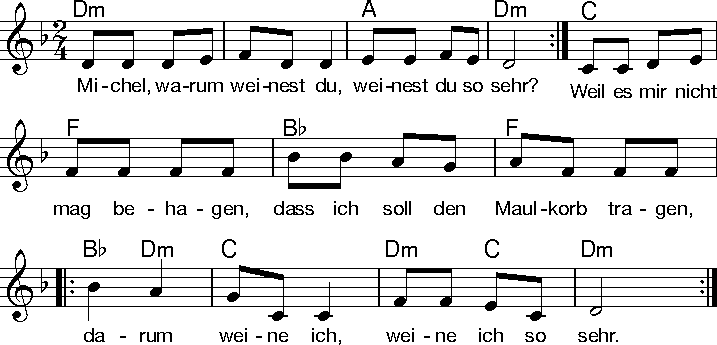
\includegraphics[draft=false, width=1\textwidth]{Noten/Lied064.pdf}	

\beginverse
\lrep\[Dm]Michel, warum weinest du, \[A]weinest du so \[Dm]sehr? \rrep
\[C]Weil sie mir mein \[F]Geld stibitzen \[B&]und es mir mit \[F]Blut bespritzen,
 \lrep\[B&]da\[Dm]rum \[C]weine ich, \[Dm]weine \[C]ich so \[Dm]sehr. \rrep
\endverse

\beginverse
\lrep^Michel, warum weinest du, ^weinest du so ^sehr? \rrep
^Weil sie mir mein ^Geld verprassen ^und nicht sagen, ^wo sie's lassen,
\lrep^da^rum ^weine ich, ^weine ^ich so ^sehr. \rrep
\endverse

\beginverse
\lrep^Michel, warum weinest du, ^weinest du so ^sehr? \rrep
^Weil ich für diese ^Ungeheuer ^Heeressteuer ^muss versteuern,
\lrep^da^rum ^weine ich, ^weine ^ich so ^sehr. \rrep
\endverse

\beginverse
\lrep^Darum, Michel, weine nun, ^weine nun nicht ^mehr!\rrep
^Wenn du einsiehst ^deine Schwächen, ^können sie dich ^nicht zerbrechen,
\lrep^da^rum ^weine nun, ^weine ^nun nicht ^mehr.\rrep
\endverse

\endsong

\beginscripture{}
Das Lied entstand kurz vor dem Revolutionsjahr 1848. Mit dem ''Michel'' ist der Deutsche Michel gemeint, eine nationale Personifikation aller Deutschen.
\endscripture
